% -*- TeX -*- -*- UK -*- -*- Soft -*-

\chapter{Processing Infrastructure}
\label{sec:ProcessingInfrastructure} 

\section{Understanding Tensor Processing Units}
\label{sec:UnderstandingTensorProcessingUnits} 

The information in this section is taken from \cite{SciForce2019}.

In 2017, Google announced a Tensor Processing Unit (TPU)---a custom application-specific integrated circuit (ASIC) built specifically for machine learning. A year later, TPUs were moved to the cloud and made open for commercial use.

Following the line of CPUs and GPUs, Tensor Processing Units (TPUs) are Google’s custom-developed application-specific integrated circuits (ASICs) that are supposed to accelerate machine learning workloads. They are designed specifically for Google’s TensorFlow framework, a symbolic math library that is used for neural networks.

TensorFlow is known to be not an easy nut to crack. To ensure a better understanding of the concept of a tensor, the TPU structure and how it works, we’ll try to give a brief and simple overview of the technology.

\subsection{What is a tensor?}

In mathematics, a tensor is a geometric object that maps geometric vectors, scalars, and other similar objects in a multi-linear manner to a resulting tensor. This may sound quite confusing, but in simpler words, a tensor is a generalized matrix that could be a 1-D matrix (a vector), a 3-D matrix (a cube of numbers), even a 0-D matrix (a single number), or a higher dimensional structure that is harder to visualize. The dimension of the tensor is called its \textit{rank}.

An important characteristic of a tensor is its dynamics: it lives in a structure and interacts with other mathematical entities. If one transforms other entities in the structure in a regular way, the tensor obeys a related transformation rule and its numerical values shirt around along with the other entities. This ``dynamical'' property of a tensor is the key that distinguishes it from a mere matrix.

In computer science, a Tensor is an n-dimensional matrix analogous to a Numpy array---the fundamental data structure used by machine learning algorithms. It is the basic unit of operation in with TensorFlow and in fact uses Numpy.

\subsection{What does it have to do with Machine Learning?}

The math involved in doing ML includes adding and multiplying these objects:

    scalar\\
    vector\\
    matrix

Let’s have a look at a simple neural network. The following example on the TensorFlow Playground \cite{GooglePlayground2019} trains a neural network to classify a data point as blue or orange based on a training dataset:

{\centering 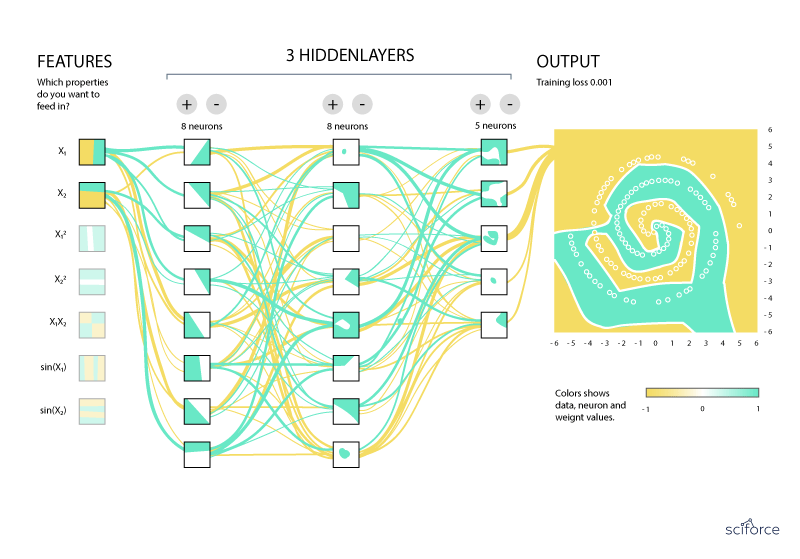
\includegraphics[width=\textwidth,]{ch0d-snip01} \par}

The trained neural network classifies data with labels or estimates missing or future values in the task called inference. For this, each neuron in a neural network undergoes the following calculations:

\begin{itemize}
\item Multiply the input data ($x$) with weights ($w$) to represent the signal strength;
\item Add the results to aggregate the neuron’s state;
\item Apply an activation function ($f$) to modulate the artificial neuron’s activity.
\end{itemize}

\begin{marginfigure}
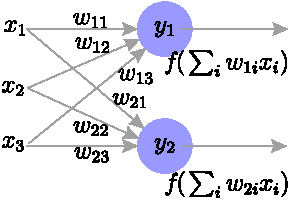
\includegraphics{chapter03-03}
\end{marginfigure}


As you can see, with three inputs and only two neurons with a fully connected single-layer neural network, you have to execute six multiplications between the weights and inputs and add up the multiplications in two groups of three. This sequence of multiplications and additions can be written as a matrix multiplication and is the most computationally intensive part of running a trained model. Every single prediction requires many steps of multiplying processed input data by a weight matrix and applying an activation function.

As a result, multiplying and taking slices from arrays takes a lot of CPU clock cycles and memory. TPUs were designed to relieve these specific workloads.

\subsection{Logic behind TPU}

To simplify the process of neural network training, TPUs address this issue in several directions.

\newthought{Quantization}

In line with the quantization technique, the process of approximation of an arbitrary value between a preset minimum and a maximum value with an 8-bit integer, TPUs contain 65,536 8-bit integer multipliers. In essence, this technique is compression of floating point calculations with 32-bit or even 16-bit numbers to 8-it integers. As you can see, the continuous large set of values (such as the real numbers) is converted to a discrete set (of integers) with maintaining the curve:

{\centering 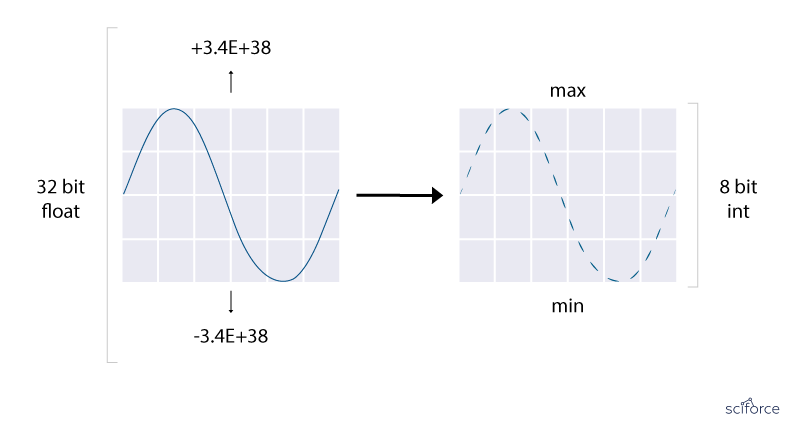
\includegraphics[width=\textwidth,]{ch0d-snip02} \par}

Quantization is the first powerful tool TPUs use to reduce the cost of neural network predictions without significant losses in accuracy.

\newthought{Focus on inference maths}

Secondly, the TPU design itself encapsulates the essence of neural network calculation. A TPU includes the following computational resources:

\begin{itemize}
\item Matrix Multiplier Unit (MXU): 65,536 8-bit multiply-and-add units for matrix operations;
\item Unified Buffer (UB): 24MB of SRAM that work as registers;
\item Activation Unit (AU): Hardwired activation functions.
\end{itemize}

They are controlled with a dozen high-level instructions that focus on the major mathematical operations required for neural network inference. A special compiler and software stack translate API calls from TensorFlow graphs into TPU instructions.

\newthought{Parallel Processing}

Typical RISC processors provide instructions for simple calculations such as multiplying by processing a single, or scalar, operation with each instruction. As you remember, a TPU contains a Matrix Multiplier Unit. It is designed as a matrix, rather than scalar, processor and processes hundreds of thousands of operations (= matrix operation) in a single clock cycle. Using such a matrix processor is like printing documents a whole page at a time rather than character-by-character or line-by-line.


\newthought{A systolic array}

The heart of the TPU is the new architecture of the MXU called a systolic array. In traditional architectures (such as CPUs or GPUs), values are stored in registers, and a program tells the Arithmetic Logic Units (ALUs) which registers to read, the operation to perform (such as an addition, multiplication or logical AND) and the register into which to put the result. A program consists of a sequence of these operations. In an MXU, matrix multiplication reuses inputs many times to procduce the final output. A value is read once but used for many different operations without storing it back to a register. The ALUs perform only multiplications and additions in fixed patterns, and wires connect adjacent ALUs, which makes them short and energy-efficient.

To understand this design, think of the heart pumping blood---like the data flowing through the chip in waves.

\begin{figure*}[tph]
%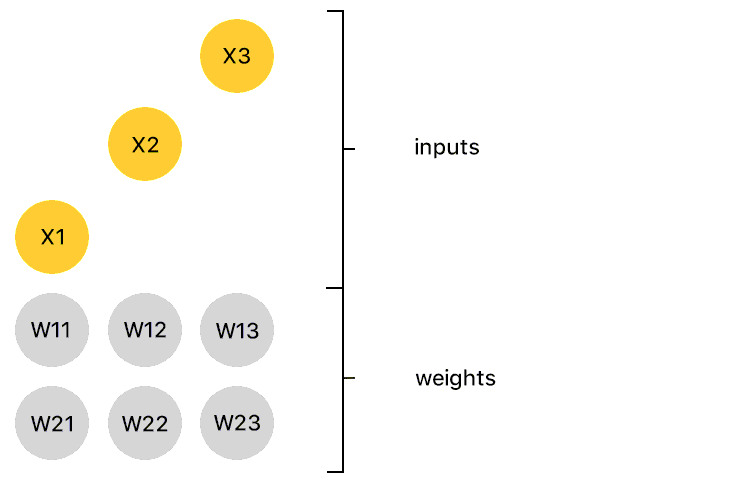
\includegraphics[width=0.3\textwidth]{tpu-waves_frame_0001}
\begin{tabular}{|c|c|c|}
\hline
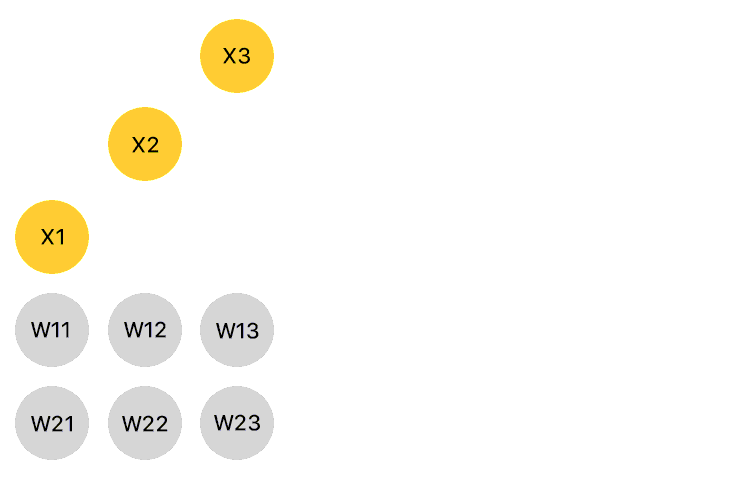
\includegraphics[width=0.25\textwidth]{tpu-waves_frame_0002}&
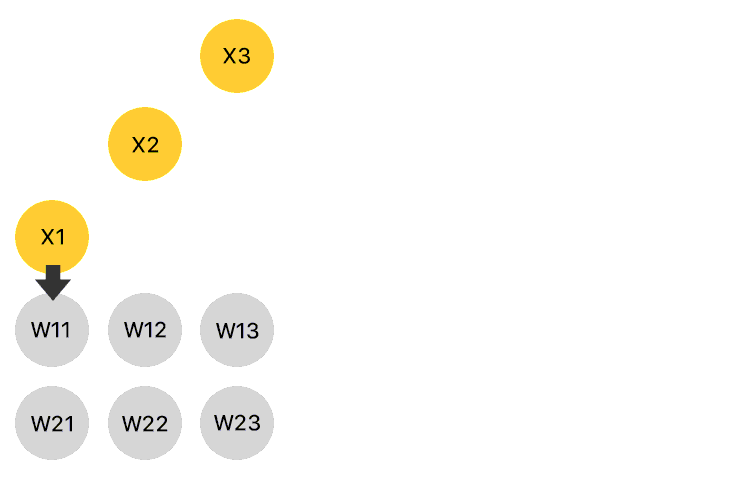
\includegraphics[width=0.25\textwidth]{tpu-waves_frame_0003}&
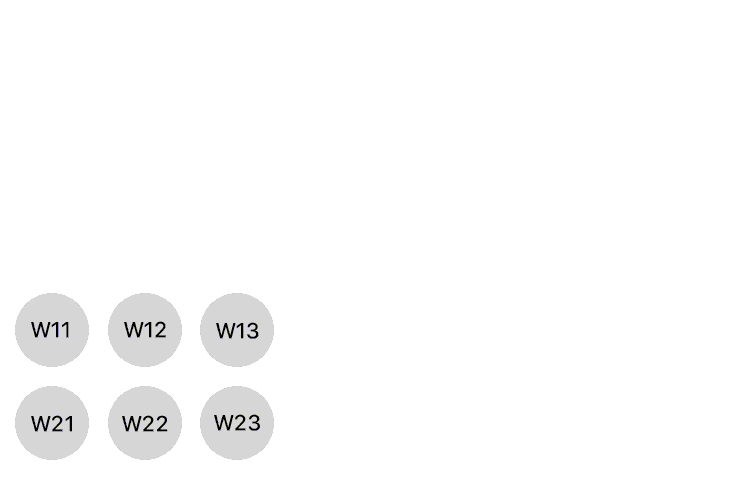
\includegraphics[width=0.25\textwidth]{tpu-waves_frame_0004}\\\hline\hline
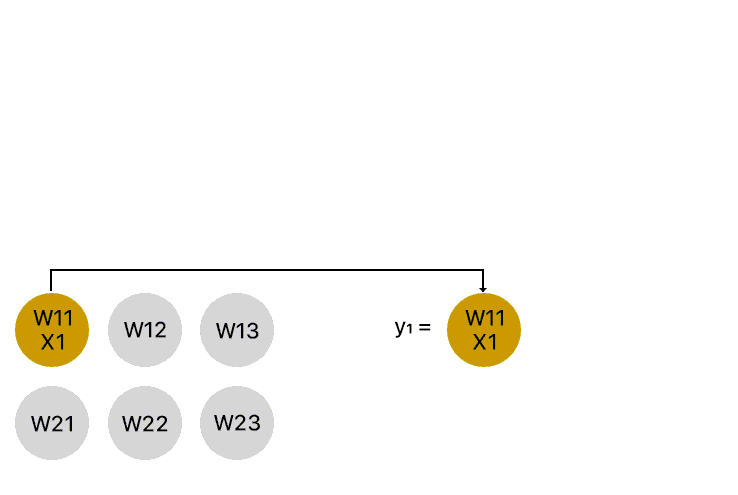
\includegraphics[width=0.25\textwidth]{tpu-waves_frame_0005}&
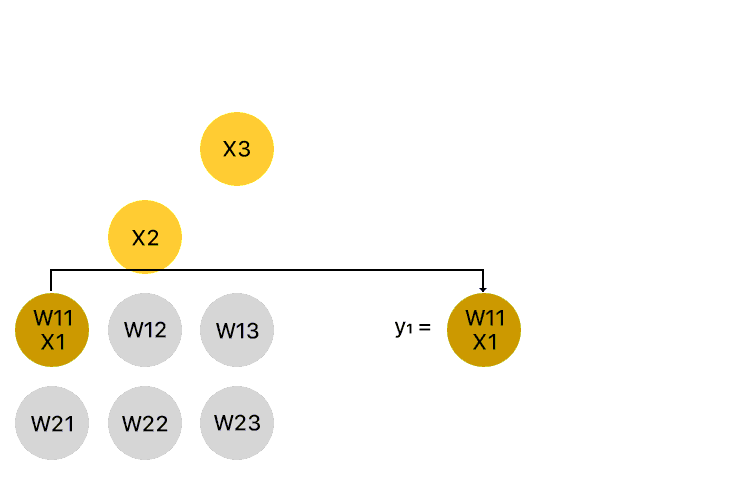
\includegraphics[width=0.25\textwidth]{tpu-waves_frame_0006}&
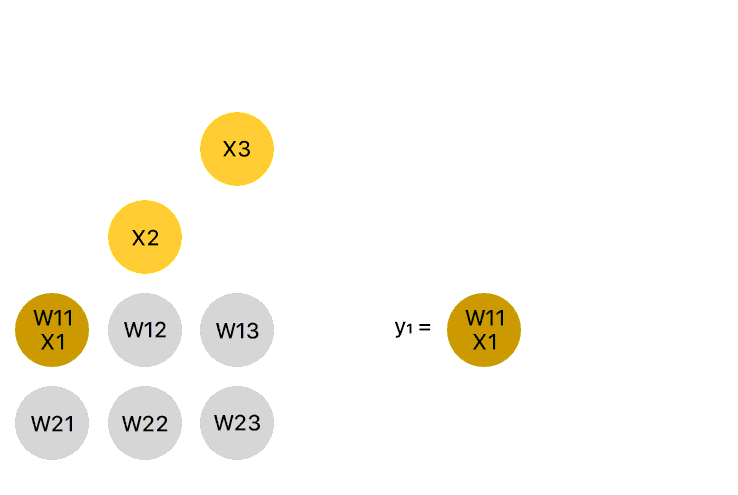
\includegraphics[width=0.25\textwidth]{tpu-waves_frame_0007}\\\hline\hline
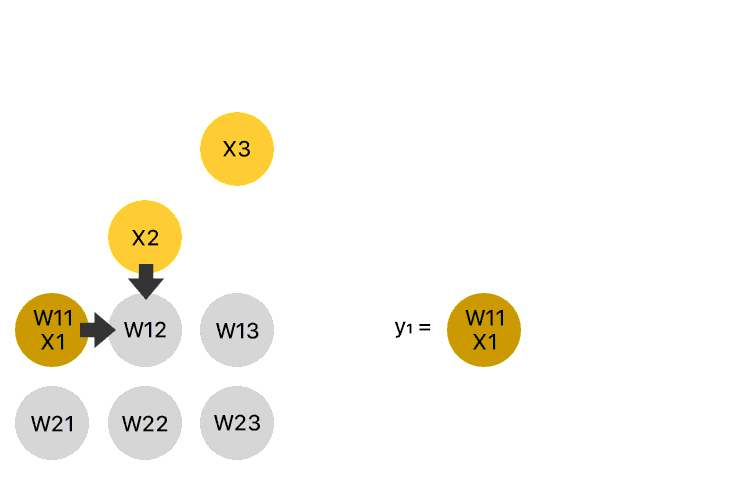
\includegraphics[width=0.25\textwidth]{tpu-waves_frame_0008}&
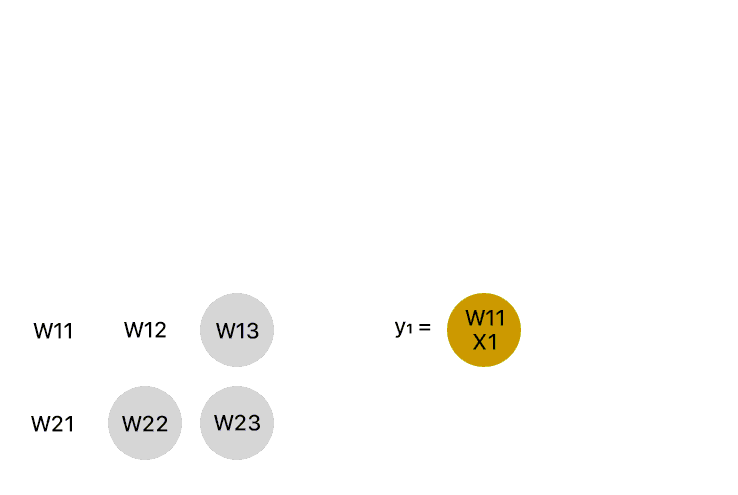
\includegraphics[width=0.25\textwidth]{tpu-waves_frame_0009}&
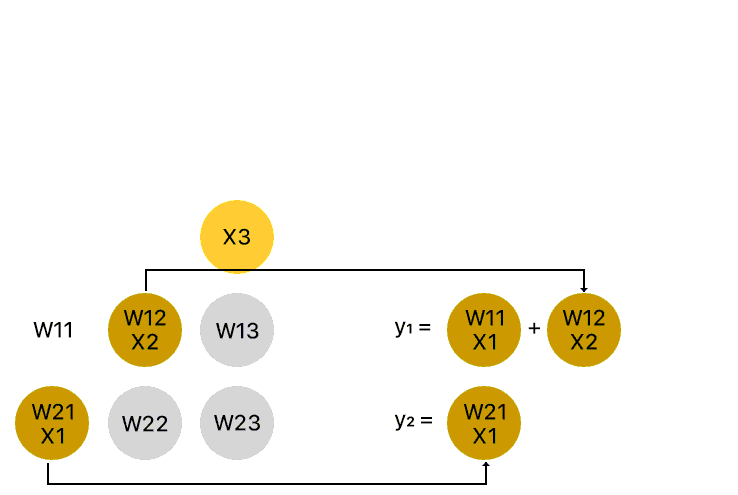
\includegraphics[width=0.25\textwidth]{tpu-waves_frame_0010}\\\hline\hline
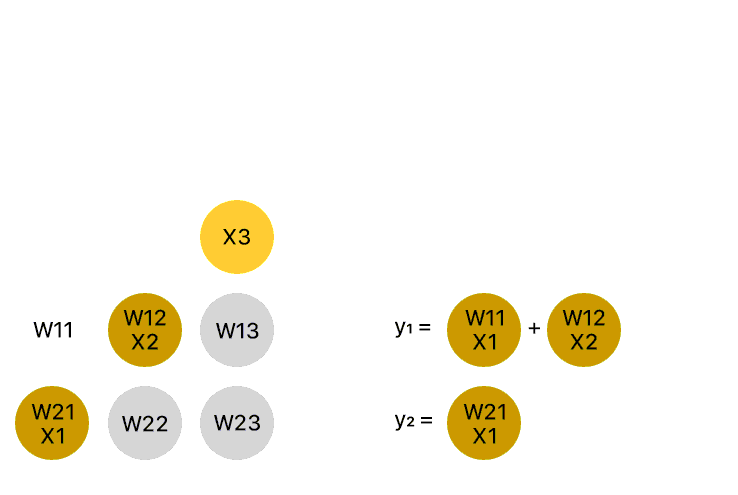
\includegraphics[width=0.25\textwidth]{tpu-waves_frame_0011}&
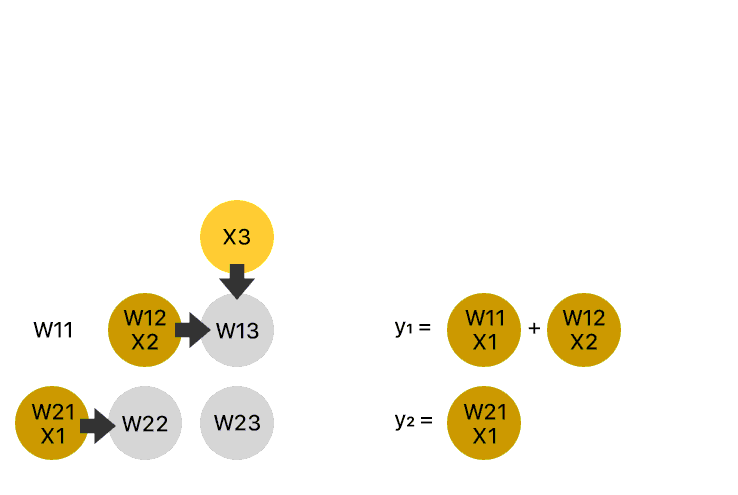
\includegraphics[width=0.25\textwidth]{tpu-waves_frame_0012}&
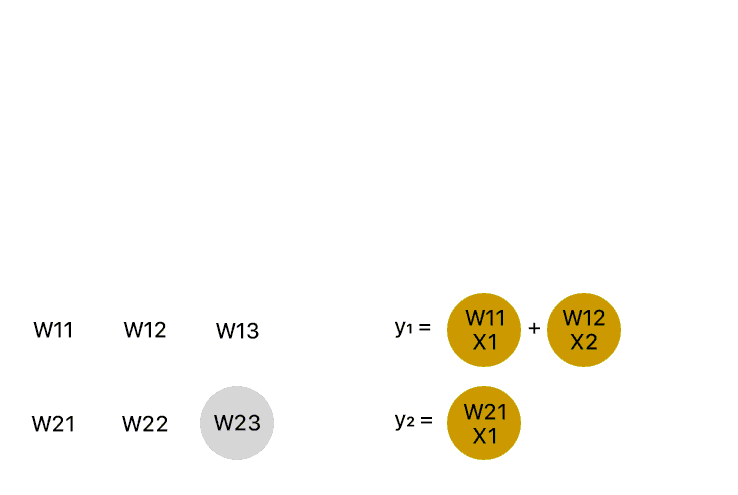
\includegraphics[width=0.25\textwidth]{tpu-waves_frame_0013}\\\hline\hline
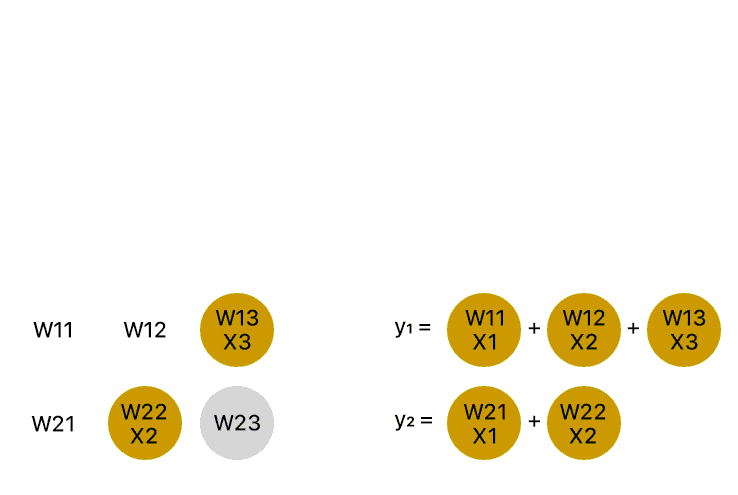
\includegraphics[width=0.25\textwidth]{tpu-waves_frame_0014}&
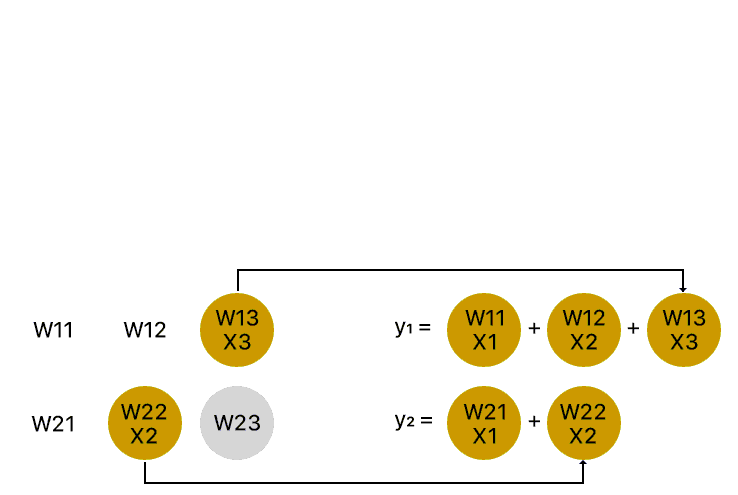
\includegraphics[width=0.25\textwidth]{tpu-waves_frame_0015}&
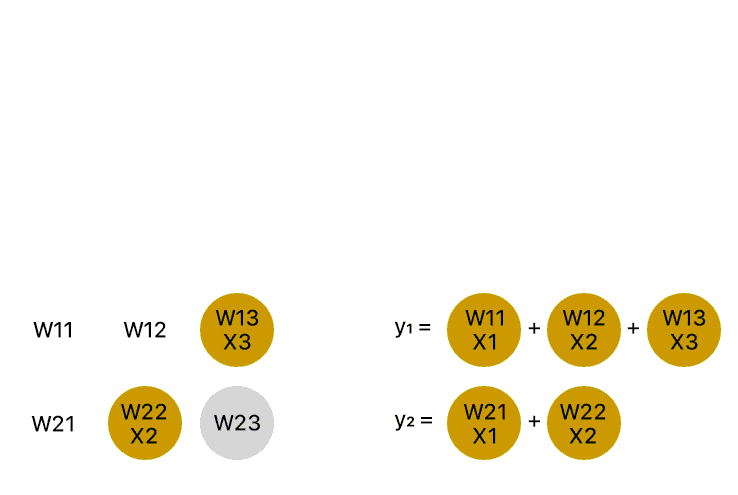
\includegraphics[width=0.25\textwidth]{tpu-waves_frame_0016}\\\hline\hline
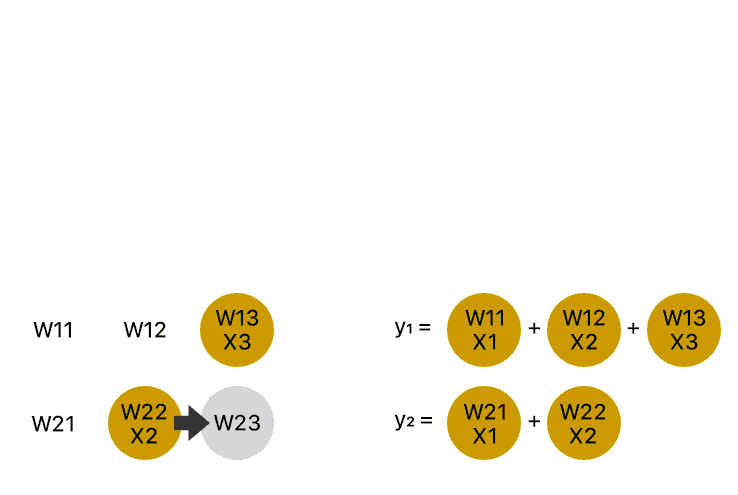
\includegraphics[width=0.25\textwidth]{tpu-waves_frame_0017}&
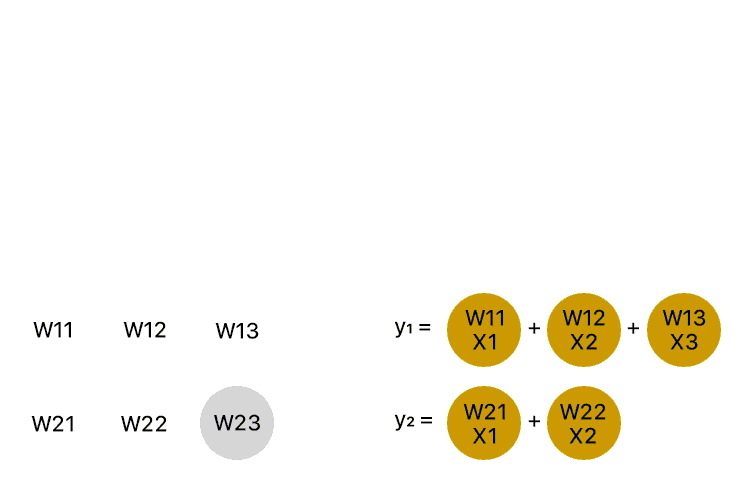
\includegraphics[width=0.25\textwidth]{tpu-waves_frame_0018}&
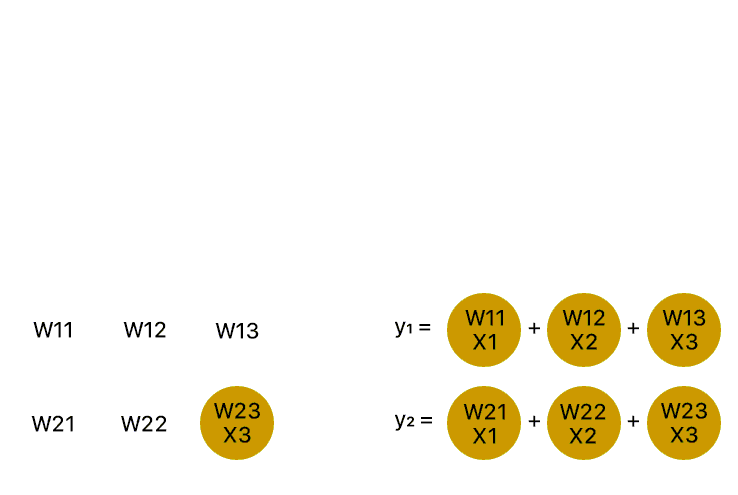
\includegraphics[width=0.25\textwidth]{tpu-waves_frame_0019}\\\hline\hline
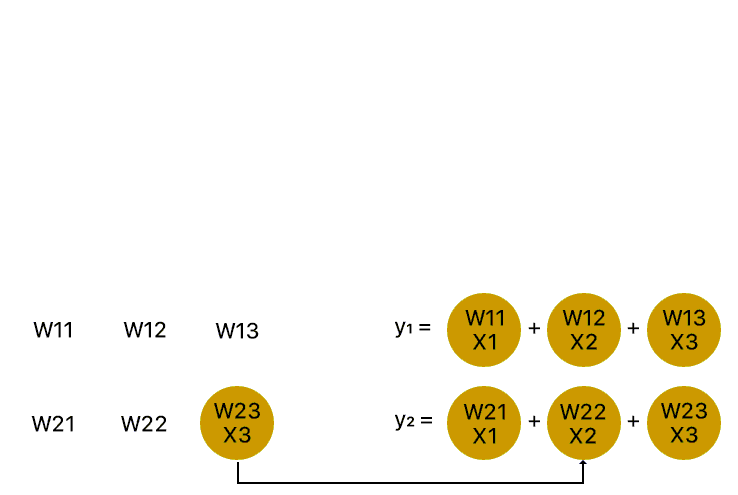
\includegraphics[width=0.25\textwidth]{tpu-waves_frame_0020}&
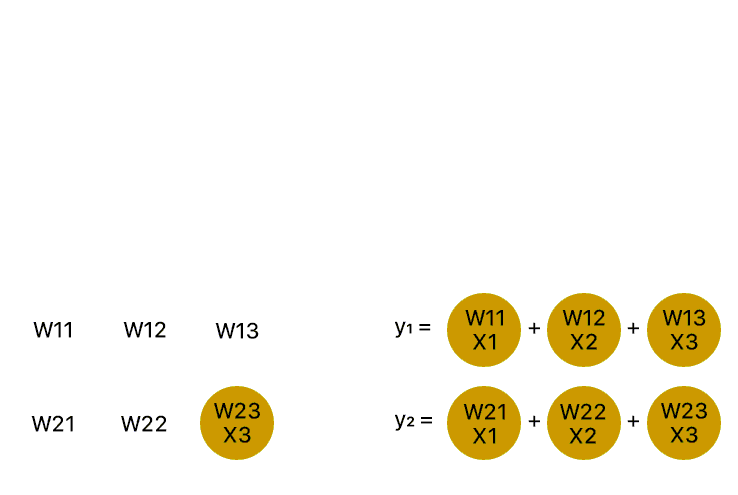
\includegraphics[width=0.25\textwidth]{tpu-waves_frame_0021}&
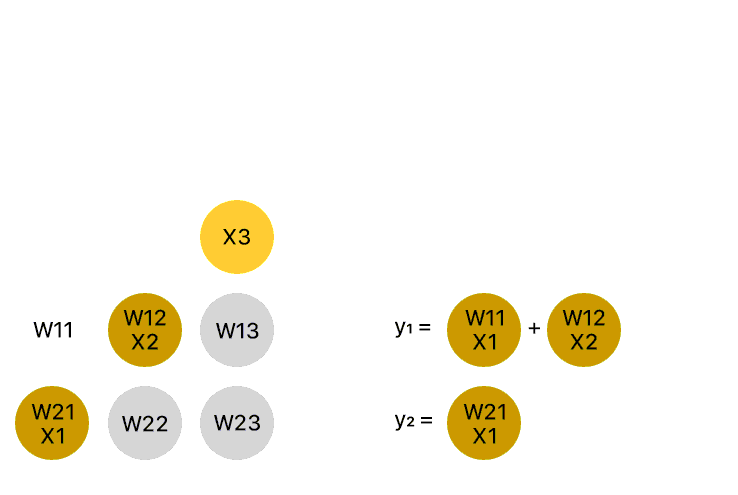
\includegraphics[width=0.25\textwidth]{tpu-waves_frame_0022}\\\hline
\end{tabular}
\end{figure*}



%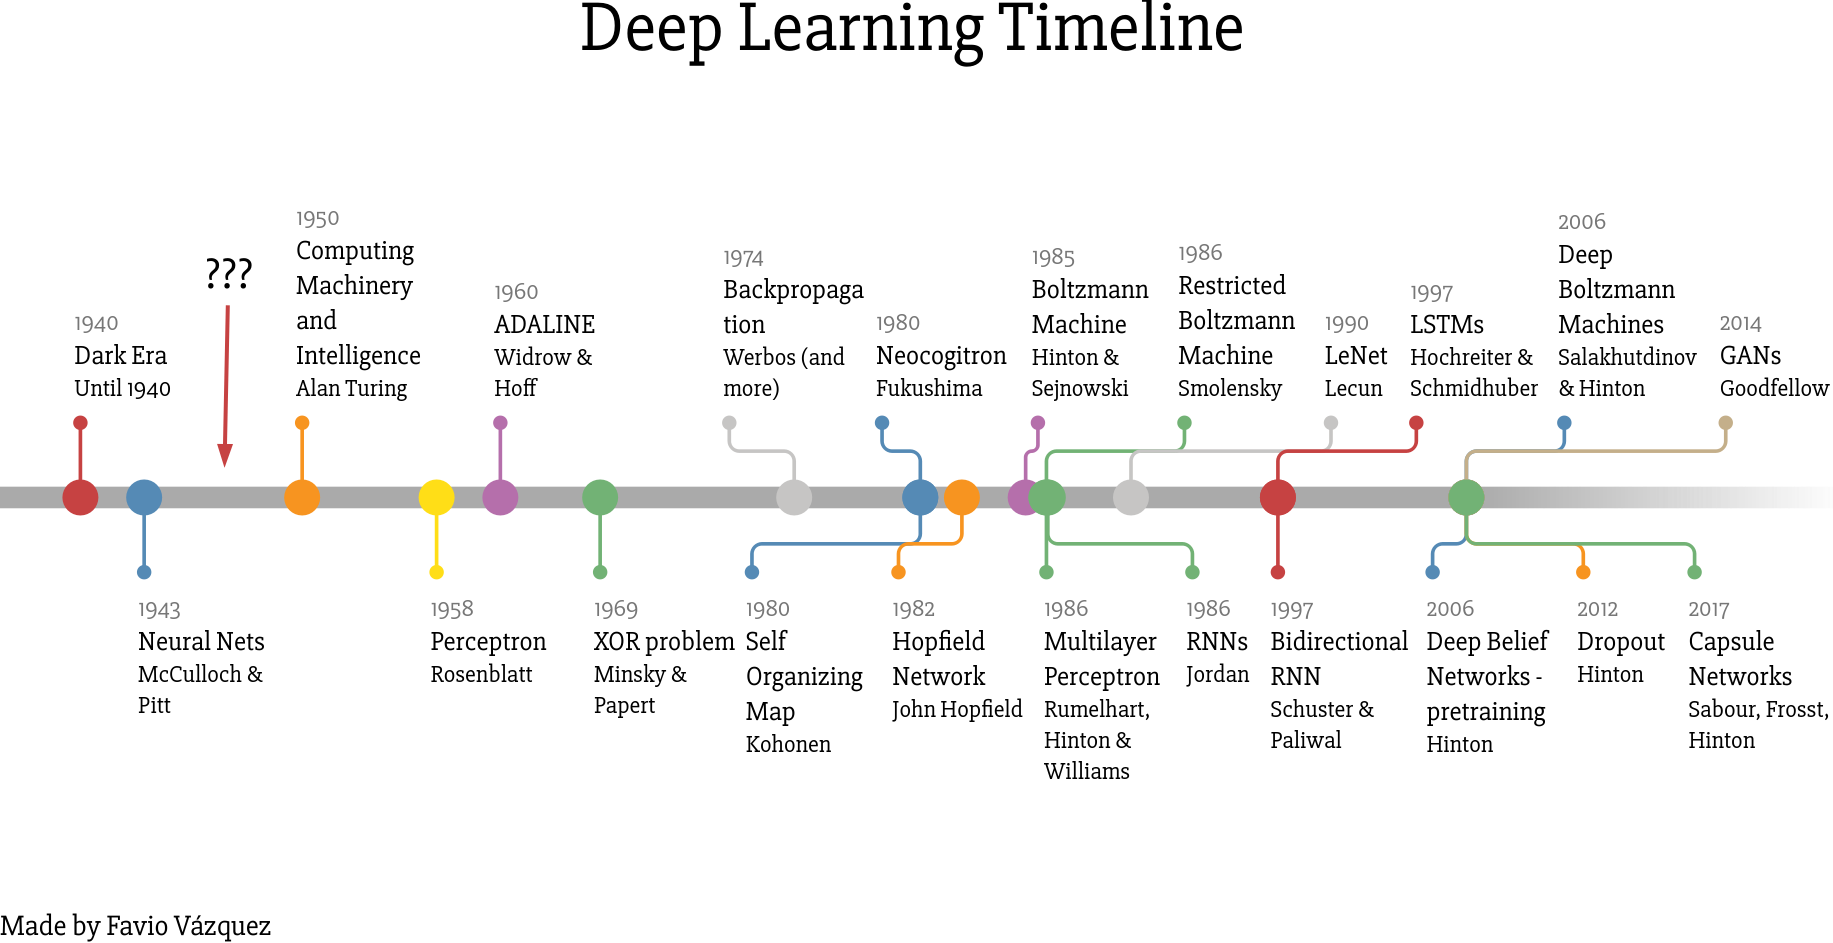
\includegraphics[width=\textwidth]{deeplearningtimeline}
%\caption{Favio V\'{a}zquez's \ac{DL} time line}
%\label{fig:deeplearningtimeline}



\subsection{Going Cloud}

Probably, the most exciting part about TPUs is that Google has made these chips available as a service on the Google Cloud Platform and shared its technology. Cloud TPU allows running machine learning workloads on Google’s TPU accelerator hardware using TensorFlow. The TPU workload is then distributed to the TPU Cloud Server, as shown below:


{\centering 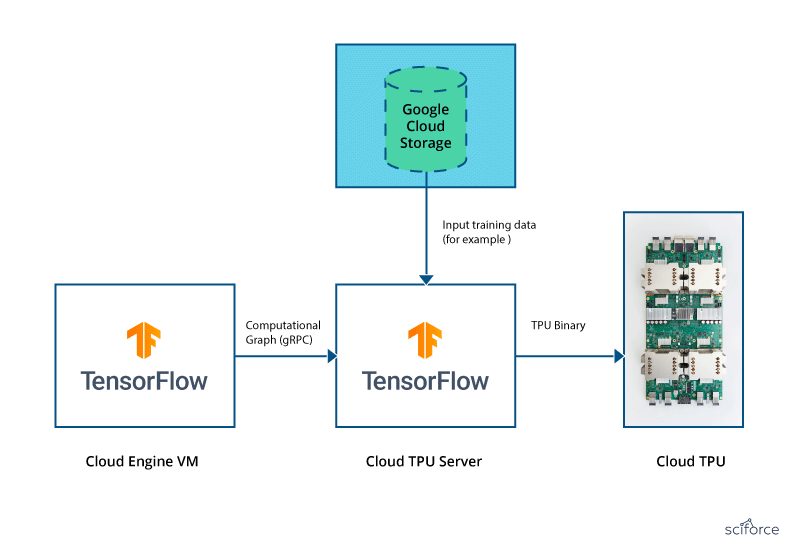
\includegraphics[width=\textwidth,]{ch0d-snip03} \par}

Cloud TPU is designed to help researchers, developers, and businesses to build TensorFlow compute clusters that can leverage CPUs, GPUs, and TPUs. High-level Tensorflow APIs help you to get models running on the Cloud TPU hardware.

\subsection{Programming model}

Transferring data between Cloud TPU and host memory is slow compared to the speed of computation because of the speed of the PCIe bus. Due to constant ‘ping-pongs’ between host and Cloud TPU, the latter is idle most of time, waiting for data to arrive over the PCIe bus. To enhance efficiency, the programming model for Cloud TPU shifts much of the training to the TPU. In this way:

\begin{enumerate}
  \item All model parameters are kept in on-chip high bandwidth memory;
  \item Many training steps are executed in a loop amortizing the cost of launching computations on Cloud TPU;
  \item The TensorFlow server fetches and pre-processes data before ``infeeding'' to the Cloud TPU hardware;
  \item Cores on a Cloud TPU synchronously execute an identical program that is stored in their own respective HBM.
\end{enumerate}

\subsection{Pricing}

According to Google’s pricing information, each TPU cost \$4.50 hour. The rates do not differ for the three TPU models shown on the website. That seems confusing as TPUs have different memory sizes and clock speeds.

\subsection{CPUs/GPUs/TPUs Contrasted}

CPUs (Central Processing Units) and GPUs (Graphics Processing Units) compute most ML problems but at the same time they consume a lot of time. Some experts contemplate that TPUs are essentially the NVidia’s GPUs moved to cloud. Since the technologies are quite similar, we offer a table contrasting the CPU, GPU and TPU chips to show how they differ and what their scopes of application are:

{\centering 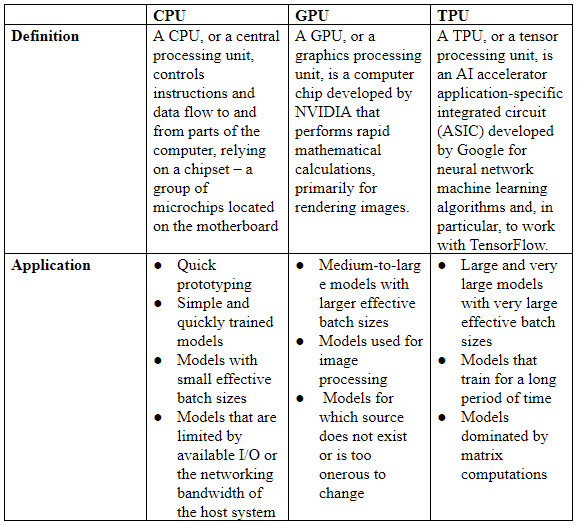
\includegraphics[width=\textwidth,]{ch0d-snip04} \par}

\subsection{Advantages of TPU}

Using TPUs offers a number of advantages in terms of increasing efficiency and speed of computation, including the following benefits:
\begin{itemize}
\item     Accelerated performance of linear algebra computation, which is used heavily in machine learning applications.
\item      Minimized time-to-accuracy when training large, complex neural network models: models that previously took weeks to train can converge in hours on TPUs.
\item      Scalable operations across different machines with their TPU servers.
\end{itemize}


\subsection{TPU Limitations}

An important thing to understand is that TPUs are specifically optimized to perform fast, bulky matrix multiplication. Cloud TPUs are likely to be outperformed by other platforms in workloads that are not dominated by matrix multiplication, such as:

\begin{itemize}
\item     Linear algebra programs that require frequent branching or are dominated element-wise by algebra;
\item     Workloads that access memory in a sparse manner;
\item     Workloads that require high-precision arithmetic;
\item     Neural network workloads that contain custom TensorFlow operations written in C++, specifically, custom operations in the body of the main training loop.
\end{itemize}

\subsection{Conclusion}

The combination of TensorFlow and TPUs can work wonders in the field of medicine, image processing and ML. When the time to train a model and the computation time are reduced from weeks to hours, machine learning becomes more competitive and available to the broader public. Besides, offering TPUs as a service on Cloud allows users to start building their models without the need of up-front capital investment. This means that researchers, engineers, small businesses and even students can start machine learning projects with ease.
